\documentclass[10pt,b5paper,tombo,openany]{jsbook}

\usepackage[dvipdfmx]{graphicx}
\usepackage[dvipdfmx]{color}
\usepackage{listings}
\usepackage{inconsolata}
\usepackage{url}
\usepackage{titlesec}
\usepackage{setspace}
\usepackage{wrapfig}

\lstset{basicstyle={\scriptsize\ttfamily}}
\lstset{breaklines=true}
\lstset{lineskip=-3pt}
\lstset{aboveskip=16pt}
\lstset{belowskip=10pt}

\renewcommand{\kanjifamilydefault}{\gtdefault}
\renewcommand{\familydefault}{\sfdefault}
\renewcommand{\contentsname}{}
\renewcommand{\baselinestretch}{0.9}

\definecolor{gray75}{gray}{0.75}
\titleformat{\chapter}[hang]{\Huge\bfseries}{\thechapter\textcolor{gray75}{|}}{0pt}{\Huge\bfseries}

\begin{document}

{\Huge OpenStackの本 --- 実践編}

\begin{minipage}{\textwidth}
	\tableofcontents
\end{minipage}

\thispagestyle{empty}

\documentclass[9pt,b5paper,tombo,openany]{jsbook}

\usepackage[dvipdfmx]{graphicx}
\usepackage{listings}
\usepackage{inconsolata}
\usepackage{url}
\usepackage{titlesec}
\usepackage[dvipdfmx]{color}
\usepackage{setspace}
\usepackage{wrapfig}

\lstset{basicstyle={\small\ttfamily}}
\lstset{frame=single}
\lstset{breaklines=true}
\lstset{lineskip=-1.5pt}
\lstset{framesep=6pt}

\renewcommand{\kanjifamilydefault}{\gtdefault}
\renewcommand{\familydefault}{\sfdefault}
\renewcommand{\contentsname}{}
\renewcommand{\baselinestretch}{1.1}

\definecolor{gray75}{gray}{0.75}
\titleformat{\chapter}[hang]{\Huge\bfseries}{\thechapter\textcolor{gray75}{|}}{0pt}{\Huge\bfseries}

\begin{document}

\noindent
{\Huge OpenStackの本 番外編}

\vspace*{-1in}
\begin{minipage}{0.4\paperwidth}
	\tableofcontents
\end{minipage}

\vspace*{1in}
\begin{minipage}{0.4\paperwidth}
	\begin{spacing}{0.75}
	\end{spacing}
\end{minipage}

\thispagestyle{empty}

\chapter{OpenStackのログに関する個人的な見解}

\setcounter{page}{1}

\marginpar{\includegraphics[width=30mm]{mini1.png}}兎にも角にもログである。これは運用するにあたって一番(ではないかもしれんが)考慮する必要がある。これをまぁいいかって感じで運用をスタートさせてしまうと、あとで地獄を見るであろう(そのほうが後学のためでもあるという意見もある)。今回は、ボク個人が至極個人的な趣味趣向とミーハー精神に基づき構築し運用もしているログのシステムについて記す。たぶん、これからOpenStackを導入する人にとっては、参考になる部分はあまり無いであろう。街談巷説、道聴塗説、話半分、そんな本章である。

\section{ログについて考えてみる}
前回出版した本 OpenStackの本 上級編ではこのように言及していた。

\begin{quotation}
  Q. 入れたはいいけど監視したいです
  A. 何を監視するか決めましょう
  まずは仮想マシンの監視ですが、これは普通のOS監視と同じ考え方で大丈夫です。ZabbixでもInfluxDBでも好きな物を使えますので、運用スタイルにあったものを選択しましょう。仮想環境ではマシンが頻繁に作成されては消えていく性質があるため、それに対応できるような監視ソリューションがいいと思います。

  コンピュートホストやネットワークノードなど、OpenStackで使われる物理サーバーの監視は普通のログやシステムメトリクスの監視に加えて、OpenStack専用の監視項目を追加する必要があるかもしれません。メモリは実使用メモリと仮想マシン割り当て量が大きく違ってきますので注意が必要です。また、ディスクもThinプロビジョニングですと、あるとき急にディスクがあふれる、なんていうこともあり得ます。libvirtのAPIなどを使用して(\verb|virsh|コマンドなど)仮想マシンホスト専用のメトリクスを取得することを考えるとよいと思います。
\end{quotation}

そう、何を監視するか、というのはとても重要である。死活監視は今回置いておくとして、監視対象のログは大きく2つに分けられる。1つ目は、イベントログ、2つ目は、パフォーマンスログである。イベントログというと、OpenStackの各コンポーネントから出力されたログである。主に、/var/log/XXX/配下にあるものを指す。パフォーマンスログとは、OpenStackの各コンポーネントを稼働させている各サーバ、及びKVMホストの性能データを指す。

これらを取得し、ストアし、分析し、障害対応のために役に立てるための定番の構成というものがある。

\begin{itemize}
  \item イベントログ (EFK, ELK stack, Splunk, etc)
  \item パフォーマンスログ (Collectd, graphite, grafana, etc)
\end{itemize}

\subsection{イベントログ}
まずは、イベントログに関して見ていこう。これについては、お金があるなら何も考えずにSplunkを導入しよう。あれは神ツールである。大規模にまで容易にスケールし、ログの構造を考えずにストアが可能で、他のツールと連携しアラートまで行えるのである。Splunkと同じことが出来る製品は他にない。Splunkを導入する予算がないのであれば、OpenStackの正確なイベントログ監視は諦めるべきである。ちなみに、経験上、Splunkそのものの運用には、ほぼ工数を割くことはない。Splunk導入は、まさにOpenStack監視における分水嶺的プロダクトといえる。

なぜ、そこまで言うのかというと、それは、OpenStackのエラーログ(及びTRACEログ)の出力にある。OpenStackは、知っての通りPythonで記述されている。つまりどういうことかというと、OpenStackのコンポーネントが何かエラーを発生させてPythonの例外処理に入った際、ログはトレース(Pythonのコールスタック)付きのCRITICALなログメッセージの形式で出力される、ということである。

この例を見ていただければ、察しがつくと思うが、このようなログをそのままログ分析用のストレージに格納し分析まで可能にするプロダクトはSplunkだけである。

\begin{lstlisting}
  2013-02-25 21:05:51 17409 CRITICAL cinder [-] Bad or unexpected response from the storage volume backend API: volume group
   cinder-volumes doesn't exist
  2013-02-25 21:05:51 17409 TRACE cinder Traceback (most recent call last):
  2013-02-25 21:05:51 17409 TRACE cinder File "/usr/bin/cinder-volume", line 48, in <module>
  2013-02-25 21:05:51 17409 TRACE cinder service.wait()
  2013-02-25 21:05:51 17409 TRACE cinder File "/usr/lib/python2.7/dist-packages/cinder/service.py", line 422, in wait
  2013-02-25 21:05:51 17409 TRACE cinder _launcher.wait()
  2013-02-25 21:05:51 17409 TRACE cinder File "/usr/lib/python2.7/dist-packages/cinder/service.py", line 127, in wait
  2013-02-25 21:05:51 17409 TRACE cinder service.wait()
  2013-02-25 21:05:51 17409 TRACE cinder File "/usr/lib/python2.7/dist-packages/eventlet/greenthread.py", line 166, in wait
  2013-02-25 21:05:51 17409 TRACE cinder return self._exit_event.wait()
  2013-02-25 21:05:51 17409 TRACE cinder File "/usr/lib/python2.7/dist-packages/eventlet/event.py", line 116, in wait
  2013-02-25 21:05:51 17409 TRACE cinder return hubs.get_hub().switch()
  2013-02-25 21:05:51 17409 TRACE cinder File "/usr/lib/python2.7/dist-packages/eventlet/hubs/hub.py", line 177, in switch
  2013-02-25 21:05:51 17409 TRACE cinder return self.greenlet.switch()
  2013-02-25 21:05:51 17409 TRACE cinder File "/usr/lib/python2.7/dist-packages/eventlet/greenthread.py", line 192, in main
  2013-02-25 21:05:51 17409 TRACE cinder result = function(*args, **kwargs)
  2013-02-25 21:05:51 17409 TRACE cinder File "/usr/lib/python2.7/dist-packages/cinder/service.py", line 88, in run_server
  2013-02-25 21:05:51 17409 TRACE cinder server.start()
  2013-02-25 21:05:51 17409 TRACE cinder File "/usr/lib/python2.7/dist-packages/cinder/service.py", line 159, in start
  2013-02-25 21:05:51 17409 TRACE cinder self.manager.init_host()
  2013-02-25 21:05:51 17409 TRACE cinder File "/usr/lib/python2.7/dist-packages/cinder/volume/manager.py", line 95,
   in init_host
  2013-02-25 21:05:51 17409 TRACE cinder self.driver.check_for_setup_error()
  2013-02-25 21:05:51 17409 TRACE cinder File "/usr/lib/python2.7/dist-packages/cinder/volume/driver.py", line 116,
   in check_for_setup_error
  2013-02-25 21:05:51 17409 TRACE cinder raise exception.VolumeBackendAPIException(data=exception_message)
  2013-02-25 21:05:51 17409 TRACE cinder VolumeBackendAPIException: Bad or unexpected response from the storage volume
   backend API: volume group cinder-volumes doesn't exist
  2013-02-25 21:05:51 17409 TRACE cinder
\end{lstlisting}

Splunkを導入できない場合、この類のログを正確に分析することは諦めよう。考えるだけ時間の無駄である。せいぜい、FluentdのFilterを駆使しまくって頑張ってくれ。


\subsection{パフォーマンスログ}
パフォーマンスログの扱いは悩ましい。いわゆる、メトリクス監視と言うものなのだが、これは一度製品選定を行うとなかなか他のものに切り替えることができないからだ。大抵の企業は、GraphiteやCollectedやSensuを駆使して監視をしているであろう。が、OpenStackを運用するような企業は比較的インフラ規模が大きくなることを見越しているはずである。前述の監視ツール群でも事足りるであろうが、個人的には、より簡単にスケールアウトさせるためにKafkaをメッセージキューとして使うことを勧めたい。なぜなら、データを転送するクライアント(= KVMホストetc)が増加すると、確実にデータを格納するストレージとの間の通信が詰まるからだ。


\section{Fluentdについて}
前のセクションでSplunkを賞賛したが、Fluentdに関しては使い所を限定すれば、とても良いプロダクトである。

\section{Kafkaについて}

\section{InfluxDBについて}

\section{OpenStack運用のためにチェックしたほうが良いログについて}

\section{KVMからVMのメトリクスを取得する方法}




\chapter{あとがき}

\setstretch{0.96}

\section*{こじろー}

\marginpar{\includegraphics[width=30mm]{mini3.png}}

\section*{まっきーさん}

\marginpar{\includegraphics[width=30mm]{mini3.png}}

\noindent
代わって檻には一匹の精悍な豹が入れられた。

\noindent
(西岡兄姉(2010)『カフカ・断食芸人』ヴィレッジブックス)

\vspace*{\stretch{1}}
\setstretch{1.0}
\begin{minipage}{0.5\paperwidth}
	著者:こじろー・まっきー

	挿絵:かとう

	発行:2016年12月31日

	印刷:POPLS (\url{http://www.inv.co.jp/~popls/})
\end{minipage}

\end{document}


\chapter{Big Tent解説}
OpenStackはそれぞれのコンポーネントが疎結合であるため、さまざまなシステムとの連携が容易であることが利点の1つです。その結果、さまざまな連携プロジェクトが生まれ、非常にリッチなクラウド環境の構築ができるようになりました。品質を維持するために、APIの仕様はきちんと議論し、それぞれのコンポーネントでリリース時期やバージョンを一致させ、相互検証を行ってきました。

が、つまりは増えすぎました。さまざまな派生プロジェクト間でのリリース調整を行うことが難しくなり、足並みをそろえるだけで大変で、開発に影響が出るようになっていまいました。そこで、OpenStackのコアとなるコンポーネントを定義し、それらの結合テスト以外はサブプロジェクトとして、リリースを一致させる必要はない、ということにしました。これをOpenStack界隈では「Big Tent構想」と呼んでいます。大きなテントにみんな一緒に、的なイメージです。

とはいえ、プロジェクトを減らそうという話ではないわけなので、相変わらずたくさんのプロジェクトが乱立しています。そんなわけで、サブプロジェクトの一部を紹介してみることにしました。プロジェクトのリストはOpenStackのWikiでまとめられているのですが、すべて英語なので調べる気が起きていない人もいるかと思います。中には単一ベンダーが1人で頑張っているだけのプロジェクトもあります。また、機能が重複しているんじゃないかというプロジェクトもあります。ちゃんとWikiが整備されていなかったり説明が無かったりと、Big Tentは玉石混交です。

図はすべてOpenStack WiKiから拝借しました。図を多く使ってドキュメントを整備してくれているプロジェクトも多く、オープンソースコミュニティの力を感じます。

\section{CloudKitty}

\begin{description}
	\item[wiki:] \url{https://wiki.openstack.org/wiki/CloudKitty}
	\item[wiki:] \url{http://docs.openstack.org/developer/cloudkitty/}
	\item[IRC:] \verb|#cloudkitty|
\end{description}

Rating-as-a-serviceと説明されていますが、課金管理をしてくれます。さまざまなメトリクスを収集し、課金ルールを定義し、ユーザーに可視化することができます。とあるITコンサルで開発されていたものをアトランタサミットでプロトタイプを紹介してみたところ、思ったより反応が良かったのでOpenStackのプロジェクトとしてオープンに開発していくことにしたようです。

一般的に課金ルールや配賦方法は、技術的というよりはビジネス的な要件から発生し、その手法もさまざまです。そのため、一般的な課金・配賦ルールはビルトインで定義されているものの、プラグイン型式で独自のルールを組み込むこともできるようになっています。Horizonとの統合も当初から設計されています。Ceilometerは確かにメトリクスを計測してくれるのですが、課金に関してはそのスコープ外でした。CloudKittyは以下のプロセスから構成されています。

\begin{itemize}
	\item 課金のもととなるデータ (collector)
	\item 課金ポリシー (rating pipeline)
	\item 課金情報の保管 (storage)
	\item 書き出し (writers)
\end{itemize}

複数のコレクターや書き出しフォーマットを選ぶことができます。

\section{Congress}

\begin{description}
	\item[wiki:] \url{https://wiki.openstack.org/wiki/Congress}
	\item[IRC:] \verb|#congress| on freenode
\end{description}

OpenStackで構成されたインフラにガバナンスを効かせるためのコンポーネントです。と、wikiには書いてありますが、イメージが掴みにくいですね。wikiの文章量はかなりあるのですが。

物理プロビジョンニングが主流だった時代と異なり、仮想的なコンピュートリソースを管理し、運用ルールを徹底させるには、その適用の自動化が必要になります。仮想マシンを1つ作るだけで毎回ファイヤーウォール設定変更の許可を書類でもらうようなことは考えたくありません。Congressはネットワークやコンピュートリソース、ネットワークリソースに対してのガバナンスフレームワークをオープンソースコミュニティで開発していこうとするプロジェクトです。例えば、

\begin{itemize}
	\item アプリケーションAはアプリケーションBとの通信のみ許可される
	\item テナントAがBグループの場合のみ、テナントAの仮想マシンはパブリックネットワークに接続される
	\item 仮想マシンAは物理的距離の遠いストレージBはマウントできない
\end{itemize}

などのルールを設定することができます。これらのルールをDatalog型式で記述します。

\section{Designate}

\begin{description}
	\item[wiki:] \url{https://wiki.openstack.org/wiki/Designate}
	\item[IRC:] \verb|#openstack-dns|
\end{description}

\begin{wrapfigure}[3]{r}[0mm]{0.3\textwidth}
	\begin{center}
		
\includegraphics[width=0.3\textwidth]{img/logo-designate.pdf}
	\end{center}
\end{wrapfigure}

みんな大好きDNSのサービスです。

\begin{itemize}
	\item ドメインとレコードの管理ができるAPIの提供
	\item マルチテナントのサポート
	\item Keystoneでの認証
	\item NovaやNeutronと連携してレコードの自動追加
\end{itemize}

いまのところPowerDNSとBIND9をインストール時点でサポートしています。プラグイン型式で追加も可能のようです。アーキテクチャはwikiで説明されています。

\begin{figure}[htb]
	\begin{center}
		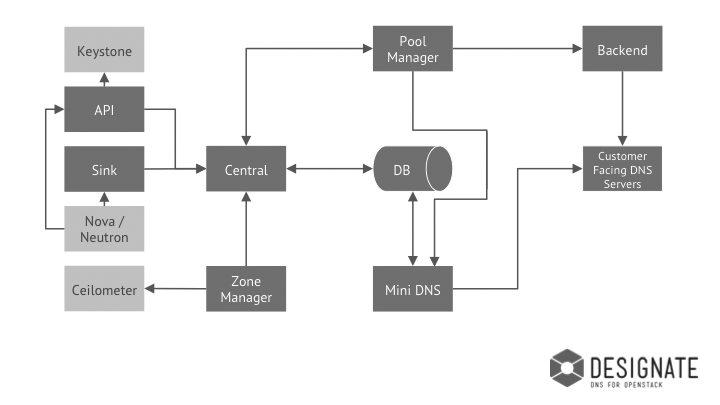
\includegraphics[width=\textwidth]{img/Designate-Arch.png}
	\end{center}
\end{figure}

\begin{description}
	\item[API:] APIリクエストを受け付けるプロセスです。認証はKeystoneへ、実際の操作はメッセージキューへ転送します。
	\item[Central:] メッセージキューからイベントを受け取ります。DNS操作を行うというよりは、Designateデータベースへの書き込みを担当します。レコード操作は別のプロセスが行います。
	\item[MiniDNS:] \verb|DNS NOTIFY|の送信や\verb|AXFR|に答えたりします。
	\item[Pool Manager:] Designate管理下にあるDNSを記憶し、同期することが責務です。
	\item[Zone Manager:] DNSの状態やゾーンの状態を定期的に監視し、Ceilometerなどに保存します。
	\item[Sink:] NovaやNeutronからのイベントを待ちます。
	\item[DNS Backend:] PowerDNS、BINDなど、実際にネームサービスを提供するサーバーです。
\end{description}

実際のコマンド例を見てみるとイメージしやすいでしょうか。ドメインの作成とレコードの作成は以下のようになるようです。

\begin{lstlisting}
$ designate domain-create --name designate-example.com. --email designate@example.org
+-------------+--------------------------------------+
| Field       | Value                                |
+-------------+--------------------------------------+
| description | None                                 |
| created_at  | 2015-02-13T16:23:26.533547           |
| updated_at  | None                                 |
| email       | designate@example.org                |
| ttl         | 3600                                 |
| serial      | 1423844606                           |
| id          | ae59d62b-d655-49a0-ab4b-ea536d845a32 |
| name        | designate-example.com.               |
+-------------+--------------------------------------+

$ designate record-create ae59d62b-d655-49a0-ab4b-ea536d845a32 --name www.designate-example.com. --type A --data 192.0.2.1
+-------------+--------------------------------------+
| Field       | Value                                |
+-------------+--------------------------------------+
| description | None                                 |
| type        | A                                    |
| created_at  | 2015-02-13T16:43:10.952601           |
| updated_at  | None                                 |
| domain_id   | ae59d62b-d655-49a0-ab4b-ea536d845a32 |
| priority    | None                                 |
| ttl         | None                                 |
| data        | 192.0.2.1                            |
| id          | 10b31f72-2358-466c-90d2-79aa015fbea4 |
| name        | www.designate-example.com.           |
+-------------+--------------------------------------+
\end{lstlisting}

プライベートDNSはなかなか自動化が進まなかったりする分野ではあるのですが、すなわちニーズもまた大きいと思います。クラウドネイティブ、という考えからするとDNSに依存するのはあまり得策ではないのですが……。とはいえやはりDNSは必要な環境も多いだろうと思うので、注目されているコンポーネントでしょう。

\section{Dragonflow}

\begin{description}
	\item[wiki:] \url{https://wiki.openstack.org/wiki/Dragonflow}
	\item[wiki:] \url{http://docs.openstack.org/developer/dragonflow/}
	\item[IRC:] \verb|#openstack-dragonflow|
\end{description}

\begin{wrapfigure}[4]{r}[0mm]{0.3\textwidth}
	\begin{center}
		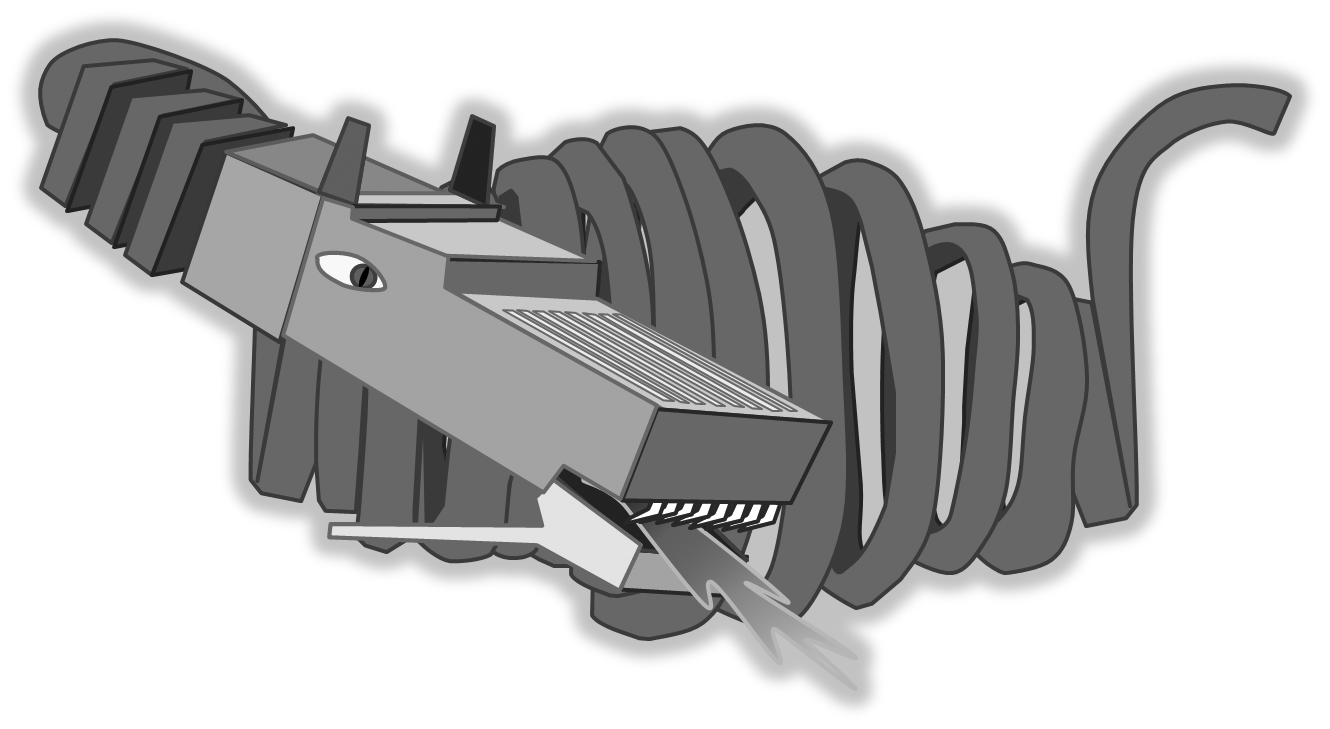
\includegraphics[width=0.3\textwidth]{img/Df_logo.png}
	\end{center}
\end{wrapfigure}

Neutron APIを使った分散型SDNコントローラー、らしいのですが、それだけ聞くとかなり壮大なプロジェクトですね。分散型のスイッチ、ルーター、DHCPなどを提供します。プロジェクトのミッションはNeutronに効率の良いシンプルなSDNを実装することです。

\begin{itemize}
	\item SDNの思想をNeutron APIに実装
	\item オープンソースコミュニティでの開発
	\item 軽量でシンプルであることをキープ。確かにNeutronのコードベースは日に日に肥大化していますからね。
	\item ネットワークのパフォーマンスに妥協しない。
	\item 分散型であることこそ至高
\end{itemize}

アーキテクチャを見ると、Open vSwitchのベースになっているようです。

\begin{figure}[htb]
	\begin{center}
		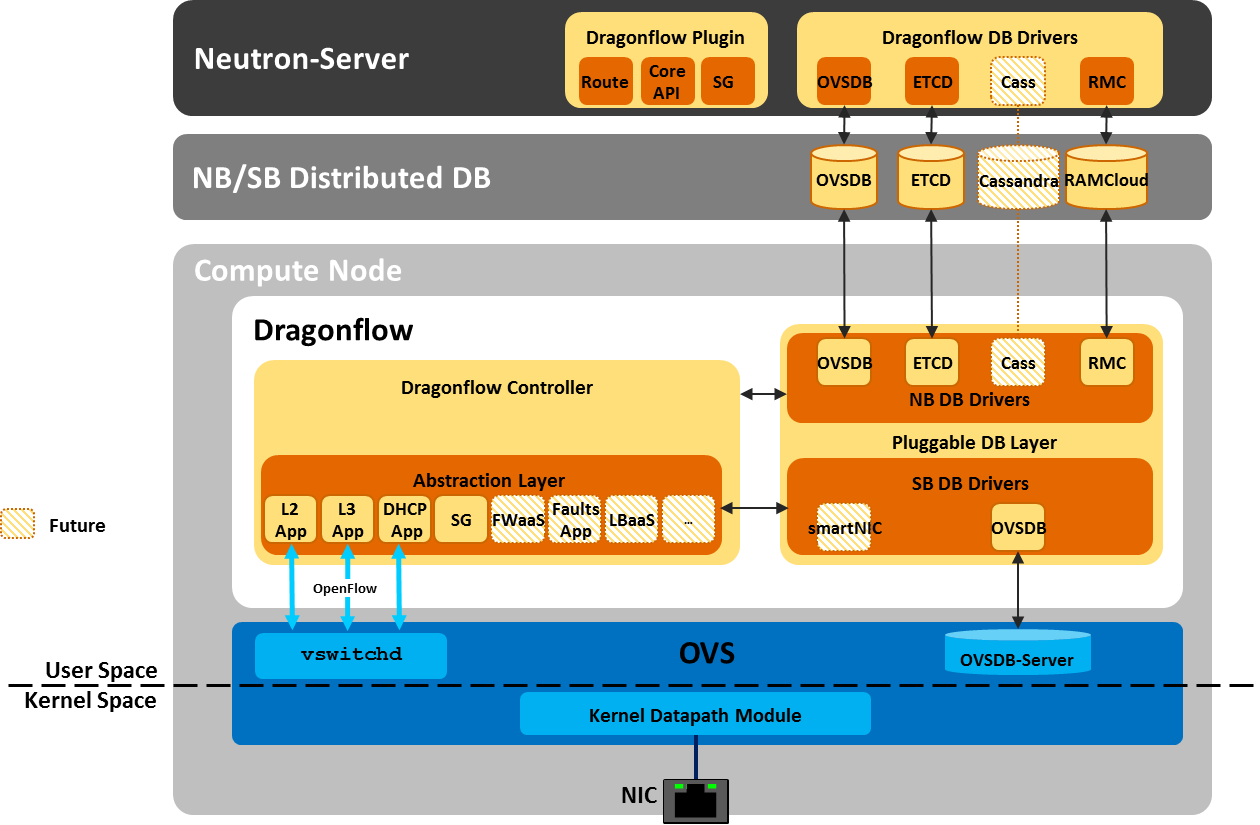
\includegraphics[width=\textwidth]{img/dragonflow_distributed_architecture.png}
	\end{center}
\end{figure}

コンテナ、NAT、障害検知などもロードマップに入っています。RJ45がドラゴンの口に見える、というのはまぁ、気持ちは分かりますが。

\section{Freezer}

\begin{description}
	\item[wiki:] \url{https://wiki.openstack.org/wiki/Freezer}
	\item[IRC:] \verb|#openstack-freezer|
\end{description}

\begin{wrapfigure}[6]{r}[0mm]{0.3\textwidth}
	\begin{center}
		
\includegraphics[width=0.25\textwidth]{img/freezer_logo.png}
	\end{center}
\end{wrapfigure}

バックアップサービスです。複数のOS(Linux・Windows・OSX・*BSD)をサポートし、ブロックストレージのバックアップやファイルシステムの差分バックアップを可能にすることが目標です。また、指定時間でのバックアップやジョブの同期など、バックアップスケジューリングも可能で、さらに暗号化もできるので安心です。さまざまなバックアップ技術が使用可能です。

\begin{itemize}
	\item セグメントサイズ(バックアップに使用するメモリ容量)
	\item キューサイズ(IOや帯域、メモリ・CPUの制限)
	\item バックアッププロセスのCPU優先度
	\item 帯域制限
	\item 暗号化(AES-256-CFB)
	\item 圧縮(zlib・bzip2・xz/lzmaなど)
	\item 並列アップロードやさまざまなストレージメディアに対応(SwiftやSSHでリモートホストへの転送など)
	\item ファイルベースの差分バックアップ(\verb|tar|など)、ブロックベースの差分バックアップ(\verb|rsync|など)
	\item マルチプラットフォーム対応(LinuxではLVMなど、WindowsではVSSに対応)
	\item 自動バックアップファイルローテーション
	\item バックアップ前後でのタスク実行
	\item 複数ノードでの同期バックアップ・リストア
\end{itemize}

Horizonとの統合も開発が進んでおり、CLIでできることがHorizonでもできるようになる予定です。以下のプロセスで構成されています。

\begin{description}
	\item[API:] REST APIの応答とスケジューラーへ受け渡しを担当します。実際のバックアップ作業は行わず、Schedulerに必要な情報を受け渡し、その結果を返すだけです。
	\item[Agent:] データをバックアップしたいリースで動くエージョンと型のプロセスです。実際にバップアップを実行します。単体で動かすこともできますが、Schedulerにより開始されることもあります。
	\item[Scheduler:] データをバックアップしたいノードで稼働する、Agentを管理するプロセスです。APIサーバーからの依頼を受け付け、バックアップ作業前後のタスクなどを担当します。Agentの動作状況を監視し、APIに返答します。並列バックアップのスケジューリングを担当します。
\end{description}

ノードで稼働するプロセスの存在が気にはなりますが、それもSSH経由などでリモートから可能であれば、十分実用可能性があると思います。オンプレ製品などにインストールするのは気が引けますね。

\section{Karbor}

\begin{description}
	\item[wiki:] \url{https://wiki.openstack.org/wiki/Karbor}
\end{description}

旧Smaugです。WikiにはOpenStackデプロイのデータとメタデータを保護するもの、あるいはKeystoneのプロジェクト下にあるものの保護、と書いてありますがこれだけではどうにもピンときません。例えば以下のようなアプリケーションがあったとします。

\begin{figure}[htb]
	\begin{center}
		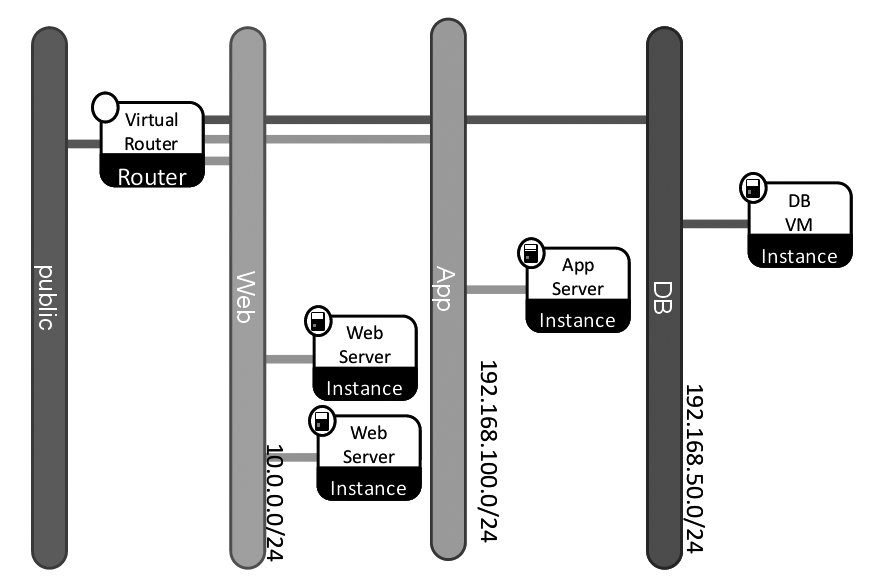
\includegraphics[width=0.7\textwidth]{img/Smaug-sample-application.png}
	\end{center}
\end{figure}

このアプリケーションをシステムまるごと保存し、変更されたことを検知したいとします。このシステムを説明すると

\begin{itemize}
	\item DBインスタンスは1つで、DBネットワークに接続されている
	\item DBネットワークはRouter配下にある
	\item Appインスタンスは1つで、Appネットワークに接続されている
	\item AppネットワークはRouter配下にある
	\item Webインスタンスは2つあり
\end{itemize}

ということになりますが、これらの情報を保存しておくことになります。Karborではこれを依存グラフとして表現します。

\begin{figure}[htb]
	\begin{center}
		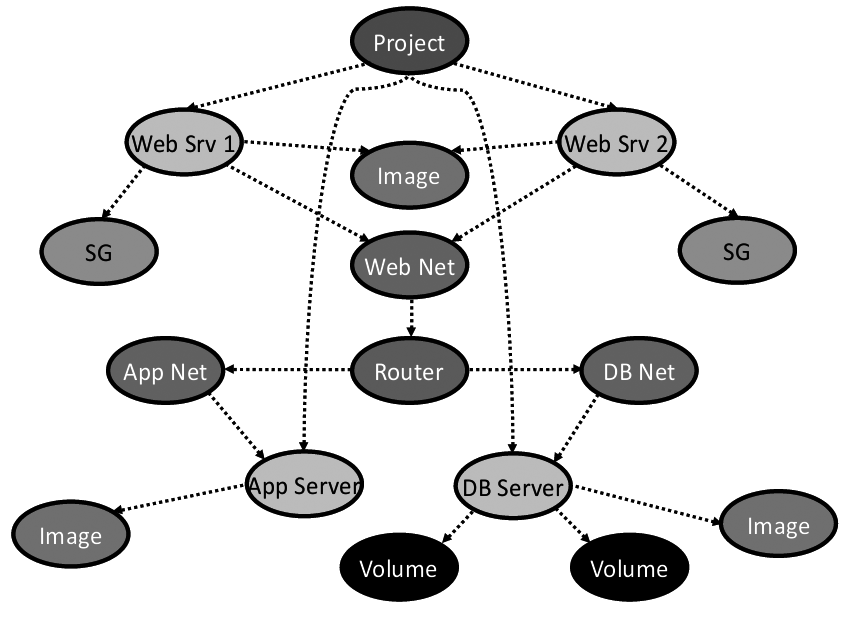
\includegraphics[width=0.7\textwidth]{img/Smaug-dependency-graph.png}
	\end{center}
\end{figure}

Wikiを見ると分かりますが、割と複雑なシステム構成になっており、デプロイするだけでも大変そうです。コンポーネントが疎結合で、組み合わせることでシステムを作っていく指向とは逆行しそうですが、まぁクラウドエンタープライズ色がかなり強いプロジェクトですね。

\section{Kolla}

\begin{description}
	\item[wiki:] \url{https://wiki.openstack.org/wiki/Kolla}
	\item[wiki:] \url{http://docs.openstack.org/developer/kolla/}
	\item[IRC:] \verb|#openstack-kolla|
\end{description}

OpenStackのコンポーネントをDocker化しようというプロジェクトです。OpenStackのAPIサーバーはImmutableなものとして扱うことが容易なので、すでにコンテナを使っている人も多いのではないかと思います。MissionにはOpenStackデプロイの簡素化や素早い増強ができるようにするとあります。

特にカスタマイズしなくても動くようなイメージを目指しているようですが、DockerfileをJinja2のテンプレートになっているのでカスタマイズが可能です。ソースコードからのインストール、RDOやUbuntuのリポジトリを使ったインストールの両方をサポートしています。コアコンポーネントだけでなく、CephやManila、Kuryrなどもデプロイできるようです。Kibanaもデプロイできるようで、これはOpenStackの監視に使う目的でしょう。

\section{Kuryr}

\begin{description}
	\item[wiki:] \url{https://wiki.openstack.org/wiki/Kuryr}
	\item[wiki:] \url{http://docs.openstack.org/developer/kuryr/}
	\item[IRC:] \verb|#openstack-kuryr|
\end{description}

\begin{wrapfigure}[10]{r}[0mm]{0.2\textwidth}
	\begin{center}
		
\includegraphics[width=0.2\textwidth]{img/kuryr_logo.png}
	\end{center}
\end{wrapfigure}

コンテナ用に設計されたNeurtonプラグインを作るプロジェクトです。Dockerのlibnetworkドライバ実装の1つという位置付けです。MagnumとNeutronの間の仲をとりもつ、という趣旨もあるようです。OpenStackを使ってコンテナのマネジメントをするために、NeutronあるいはDockerコミュニティーに対して必要な働きかけ行ったりもするようです。Kuryr自体がコンテナネットワーク実装の唯一解になるつもりはないそうです。

コンテナに関しては長らくすったもんだを繰り返していましたが、ネットワークはKuryrになんとか落ち着いていきそうです。コンテナ自体はMagnumで落ち着きそうですし、OpenStackとコンテナはなんとか落としどころを見つけたのでしょうか。そもそも、仮想マシン(インスタンス)とコンテナではライフサイクルが違う、ということに無理があったりはします。

ところで、どう発音すればよいのかは謎である。くりあー?くりゅあー?

\section{Monasca}

\begin{description}
	\item[wiki:] \url{https://wiki.openstack.org/wiki/Monasca}
	\item[IRC:] \verb|#openstack-monasca|
\end{description}

インスタンスのモニタリングし、アラートを出してくれるようなサービスを作るプロジェクトです。高可用性とスケーラビリティーの良さをうたっており、OPNFVからの注目が熱いプロジェクトです。以下のような特徴を持っています。

\begin{itemize}
	\item ハイパフォーマンス・スケーラブル・高可用
	\item REST API実装によるシンプルな動作
	\item マルチテナント対応
	\item リアルタイム性
	\item 複数のアラームの合成
	\item Nagiosや\verb|statsd|との連携
	\item オープンコミュニティーでの開発
\end{itemize}

構成は意外と複雑です。

\begin{figure}[htb]
	\begin{center}
		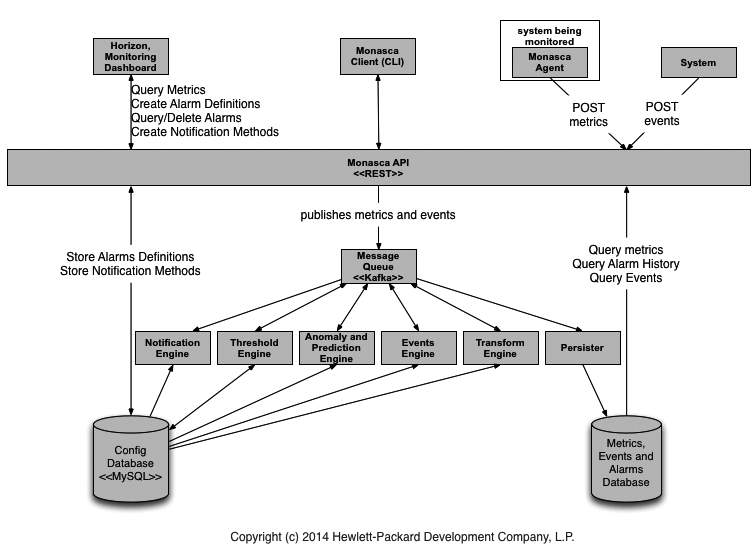
\includegraphics[width=\textwidth]{img/Monasca-arch-component-diagram.png}
	\end{center}
\end{figure}

\begin{description}
	\item[Agent:] メトリクス監視エージェントです。MySQLなど有名所に対してはデフォルトである程度のアラートセットを定義済みです。Nagiosや\verb|statsd|との連携もできます。
	\item[Persister:] メッセージキューからのデータをデータベースに保管することに特化したプロセスです。大量のデータを高速に処理する必要があるので分離されているのでしょう。
	\item[UI:] Horizonに統合されています。モニタリングにはやはりGUIがあるべきでしょう。
	\item[Ceilometer Publisher:] Ceilometerとの連携機能もあります。
\end{description}

可用性とパフォーマンスにはかなり気を遣っているようです。既存のモニタリングシステムとの連携も考えられているようなので、段階的な導入はできそうな気がします。

\section{Searchlight}

\begin{description}
	\item[wiki:] \url{https://wiki.openstack.org/wiki/Searchlight}
	\item[wiki:] \url{http://docs.openstack.org/developer/searchlight/}
	\item[IRC:] \verb|#openstack-searchlight|
\end{description}

確か最初はGlanceのイメージを検索できるように、というような趣旨のプロジェクトだった気がするのですが、LibertyでのデザインサミットでGlanceに限らずOpenStackのリソースすべてを検索対象とする方針の転換がありました。今はサーチサービスという大義のようです。ミッションは「マルチテナンシーのある、スケーラブルなインデクサーとサーチエンジンの提供」です。

\begin{figure}[htb]
	\begin{center}
		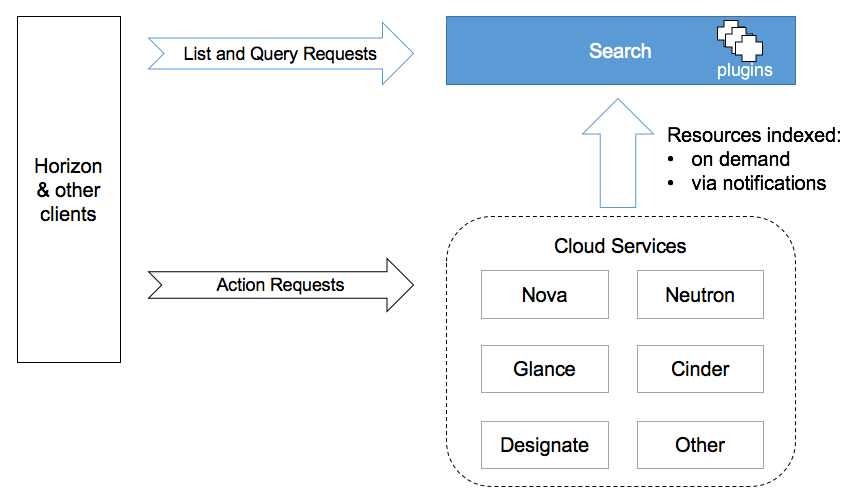
\includegraphics[width=\textwidth]{img/Searchlight-Concept-1.png}
	\end{center}
\end{figure}

OpenStackにかかわるあらゆるもの、例えばインスタンスなどの情報を集めて、Elasticsearchにインデックスし、それを検索可能にするAPIを提供します。Horizonのインスタンス検索機能は貧弱ですし、APIも文字列部分一致程度のリスティング機能しかありませんので、Searchlightは便利だと言えるでしょう。

\section{Senlin}

\begin{description}
	\item[wiki:] \url{https://wiki.openstack.org/wiki/Senlin}
	\item[wiki:] \url{http://docs.openstack.org/developer/senlin/developer/index.html}
	\item[IRC:] \verb|#senlin|
\end{description}

インスタンスをクラスタ化することができるAPIを提供します。Novaが作成したインスタンスだけが対象ではなく、Heatのスタックなどもクラスタ化することができます。Heatで頑張ればなんとかできる、をSenlinでちゃんとやる、という感じです。

以下のような構成で動作します。

\begin{figure}[htb]
	\begin{center}
		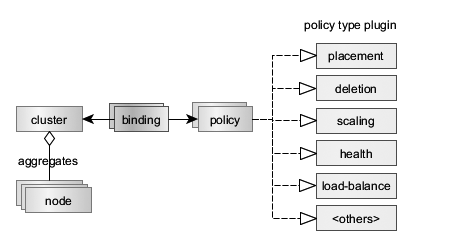
\includegraphics[width=\textwidth]{img/Senlin-policies.png}
	\end{center}
\end{figure}

クラスタを管理するにおいて、ポリシーを設定することができ、以下のプラグインがあるようです

\begin{itemize}
	\item 配置 (Placement)
	\item 削除 (Deletion)
	\item スケール (Scaling)
	\item ヘルスチェック (Health)
	\item ロードバランシング
	\item その他
\end{itemize}

これらのポリシーに紐付けられたノードをまとめて管理することでクラスタを生成します。

\section{Solum}

\begin{description}
	\item[wiki:] \url{https://wiki.openstack.org/wiki/Solum}
	\item[wiki:] \url{http://docs.openstack.org/developer/solum/index.html}
	\item[IRC:] \verb|#solum|
\end{description}

Software Development Lifecycle Automation service: 直訳するとソフトウエア開発サイクルの自動化サービス、です。ソースコードのOSイメージへの配置やデプロイ作業を自動化し、OpenStackをアプリケーション開発フローと統合させることがミッションです。

プロジェクトのゴールは開発者目線からとアプリケーションの可搬性、アプリケーションを作成するプログラミング言語に依存しない設計の3つから定められています。

\subsection*{開発者の生産性}
\begin{itemize}
	\item 開発・テスト・ステージング・本番、などの環境を意識できるアプリケーションサイクルの管理ができる
	\item 自動化されたデプロイフローによるCI/CD環境の構築
	\item \verb|git push|
	\item IDE連携
\end{itemize}

\subsection*{アプリケーションの可搬性}
\begin{itemize}
	\item Solumnで動くアプリケーションは、どのベンダーのOpenStackでも動く
	\item パブリッククラウドでもプライベートクラウドでも動く
	\item Novaベースでデザインされているため、Dockerに対応
\end{itemize}

\subsection*{言語・拡張性}
\begin{itemize}
	\item ランタイムをプラグイン形式にすることで、Solumn自体はアプリケーションを作成したのプログラミング言語に依存しない。
	\item アドオン型式なので、独自の拡張が可能
	\item つまり、ベンダー独自の拡張も可能ではある
\end{itemize}

NovaのDokcerを使う、という辺りに少し不安はあるものの、ニーズは大きそうなプロジェクトです。

\section{Vitrage}

\begin{description}
	\item[wiki:] \url{https://wiki.openstack.org/wiki/Vitrage}
	\item[wiki:] \url{https://github.com/openstack/vitrage/tree/master/doc/source}
	\item[IRC:] \verb|#openstack-vitrage|
\end{description}

\begin{wrapfigure}[9]{r}[0mm]{0.3\textwidth}
	\begin{center}
		
\includegraphics[width=0.3\textwidth]{img/Vitrage_logo_finaly.png}
	\end{center}
\end{wrapfigure}

OpenStackのアラートやイベントを可視化したり分析することで、トラブルを未然に防いだり、トラブルシューティングに役立てようとするプロジェクトです。以下のような機能を持っています。

\begin{itemize}
	\item コンピュートホストやネットワーク機器などの物理機器の状態と、その物理機に依存している仮想マシンとの紐付け
	\item 直接OpenStackを監視するのではなく、システムの分析をベースにした状態の変化やアラーティング
	\item アラートやイベントによる問題解決
	\item ダッシュボード (Horizon)
\end{itemize}

アーキテクチャは以下のようになっています。

\begin{figure}[htb]
	\begin{center}
		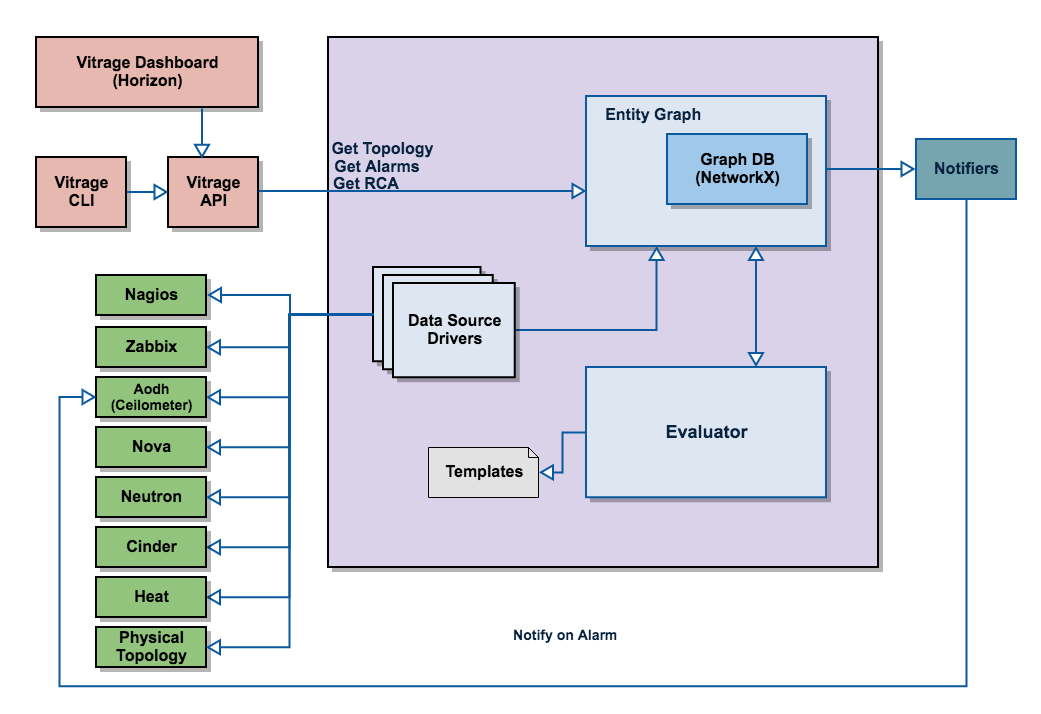
\includegraphics[width=\textwidth]{img/Vitrage-high_level_architecture2.png}
	\end{center}
\end{figure}

とあるネットワークスイッチで障害が発生した場合、どの仮想マシンが影響を受けるか、といった分析が可能になります。これらの情報を持っていることで、物理機器のメンテナンス時の影響を把握することも簡単になりそうです。

\section{Watcher}

\begin{description}
	\item[wiki:] \url{https://wiki.openstack.org/wiki/Watcher}
	\item[wiki:] \url{http://docs.openstack.org/developer/watcher/index.html}
	\item[IRC:] \verb|#openstack-watcher|
\end{description}

OpenStackベースのクラウド環境でのリソース制御機構を提供しようというプロジェクトです。システムメトリクスの収集や最適化、アクションプランのプロセスが動作します。データセンターの運用コストやマイグレーションによるシステムパフォーマンスの改善、電源効率の改善なども視野に入っているようです。制御アルゴリズムはデフォルトで入っているもの以外にもプラグイン形式で追加することもできます。OpenStack運用者のためのプロジェクトと言えます。なんともピンと来ませんが、いくつがユースケースが紹介されています。

\begin{itemize}
	\item サーバー筐体の温度や空調、電源管理などの物理的なリソースの運用時に、仮想マシンのホスト間移動や適切なスケジューリングの機構を提供する
	\item 最適化が必要になるしきい値の指定や変更が容易になる
	\item テストや開発環境ではリソースを詰めて、本番環境では少し余裕を持たせたスケジューリングをしたいなど、リソースセットを定義する
	\item リソースの使用状況を詳細に監視する
	\item イベントにはOpenStackのあらゆるコンポーネントに対応可能。 (Novaのマイグレーション、Keystoneの認証など)
	\item 逆にWatcherからイベントを発行させることも可能
\end{itemize}

以下のアーキテクチャで動作しています。例によって、メッセージキューによるイベント駆動になっています。また、データベースが2つあるようです。

\begin{figure}[htb]
	\begin{center}
		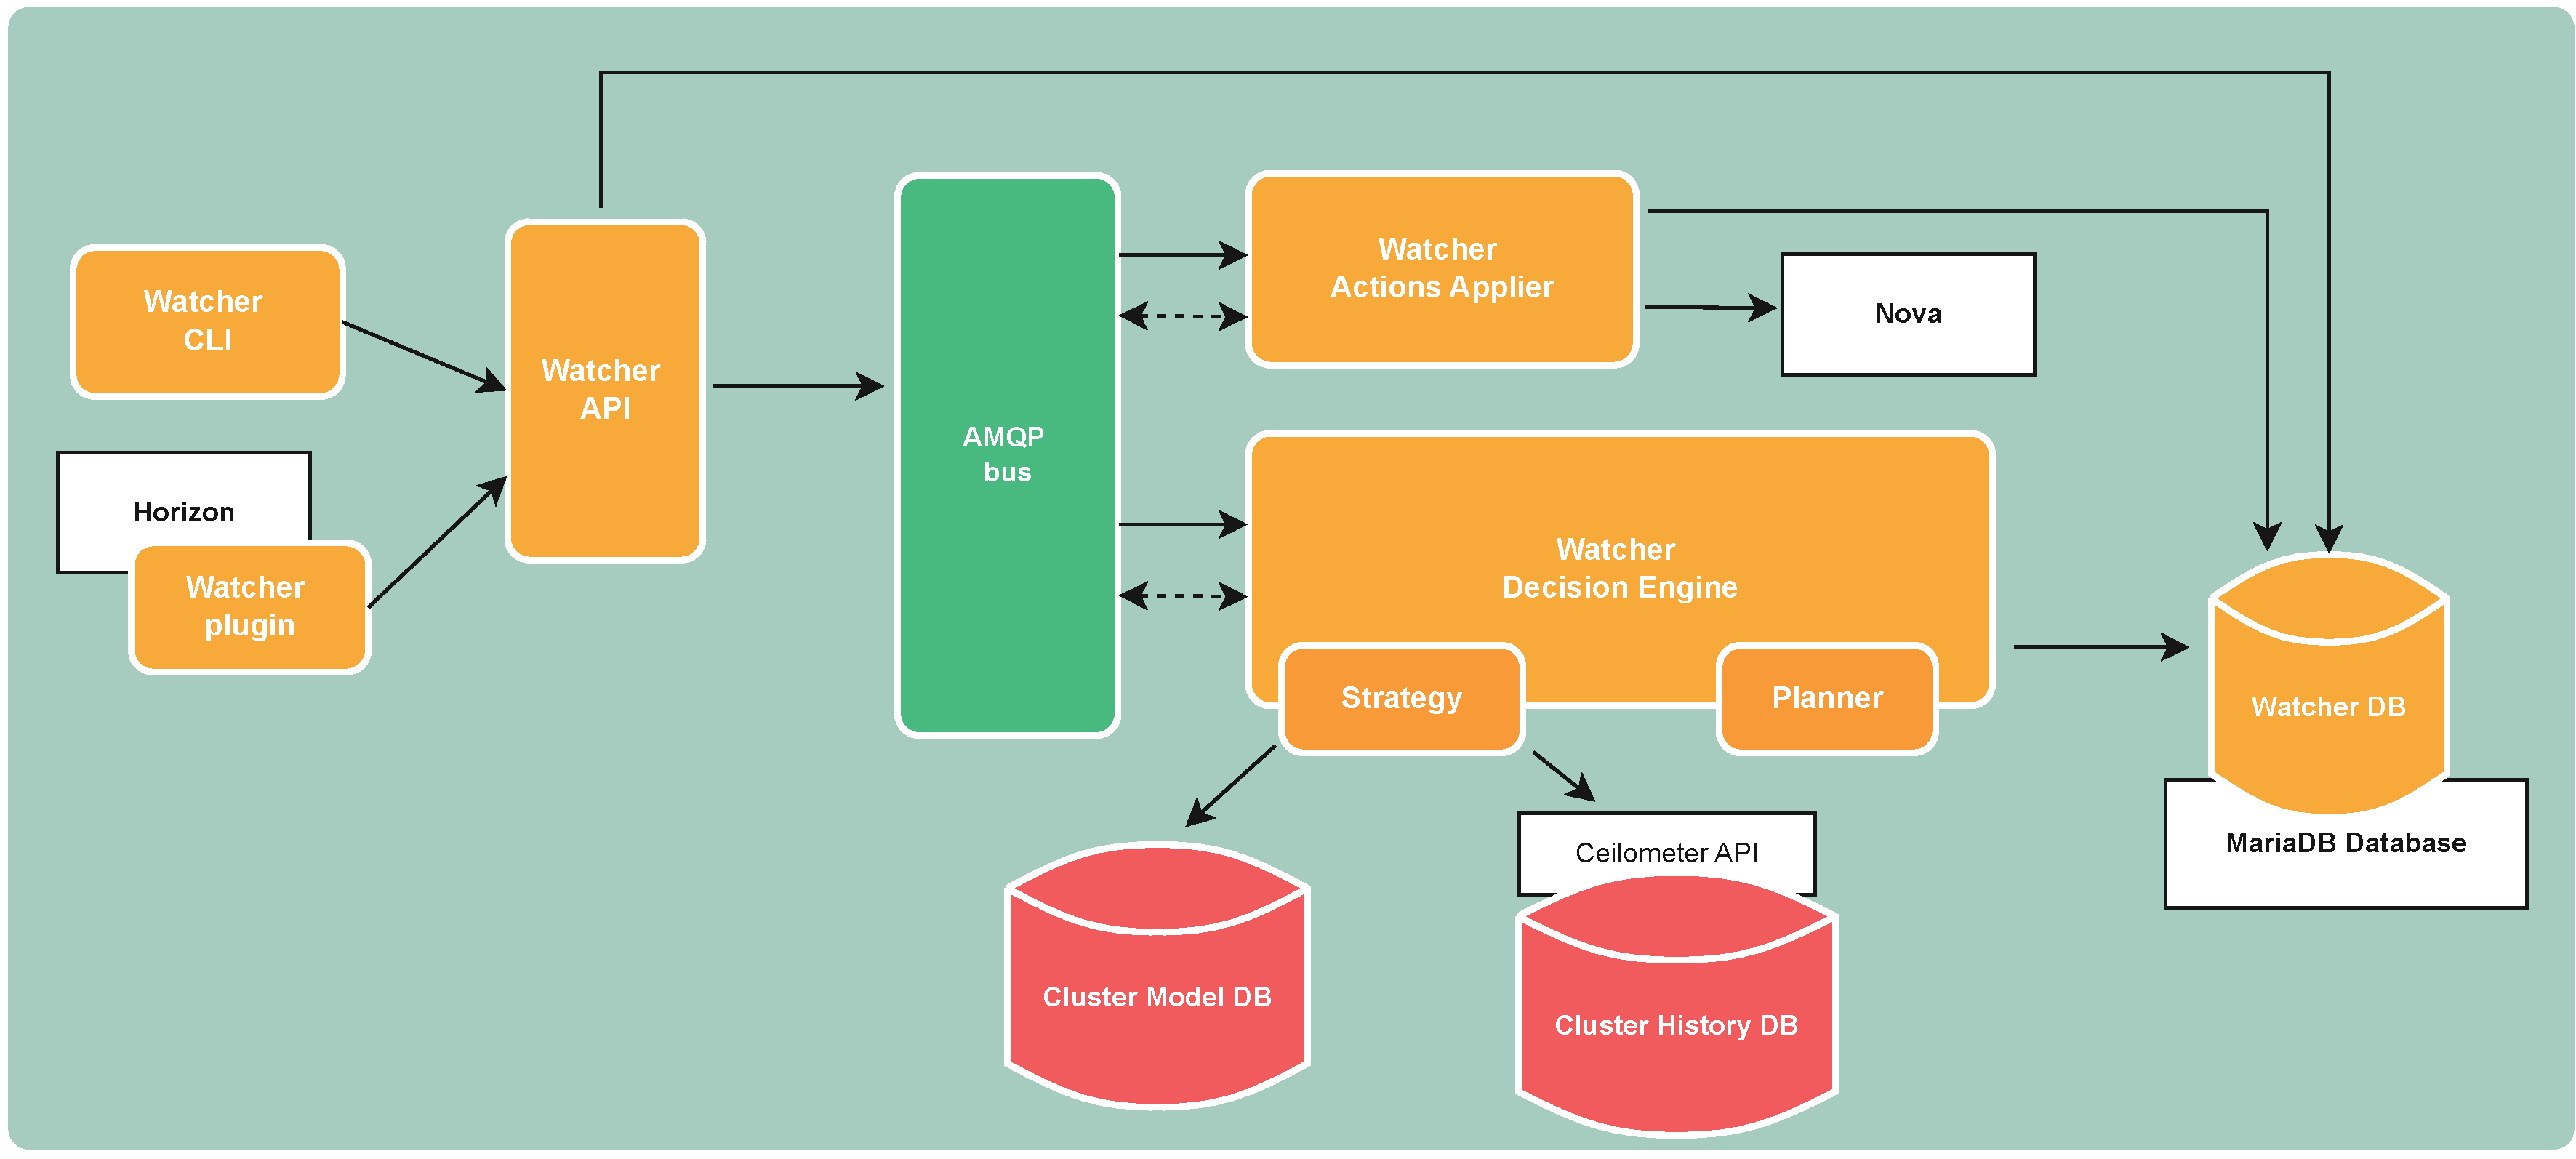
\includegraphics[width=\textwidth]{img/watcher-architecture.pdf}
	\end{center}
\end{figure}

\begin{description}
	\item[API:] REST API実装です。実際のタスクは行いません。
	\item[Decision Engine:] Applierに渡すActionを作成します。「あるべき姿」にシステムを収束させるためのタスクを決定するプロセスになります。
	\item[Applier:] メッセージバスに接続され、Decision Engineが作成したプランを実際にプランを実行するプロセスです。タスクの失敗・成功を通知する機能があります。
	\item[Database:] Cluster History DBにはクラスタのメトリクスが保管されます。Ceilometerと似ています。Cluster Model DBにクラスタの情報は保管されるようです。
\end{description}

いかがだったでしょうか。OpenStackの懐の広さを感じてもらえたかと思います。実は他にもマイナーなプロジェクトがあったり、OpenStackの開発インフラを使用しないプロジェクトなんかもあったりしますので、いろいろ見てみると楽しいと思います。


\chapter{あとがき}

\vspace*{\stretch{1}}
\setstretch{1.0}
\begin{minipage}{0.5\paperwidth}
	\begin{description}
		\item[著者:]こじろー・まっきー
		\item[挿絵:]かとう
		\item[発行:]2016年12月31日
		\item[印刷:]POPLS (\url{http://www.inv.co.jp/~popls/})
	\end{description}
\end{minipage}

\end{document}
